\documentclass{article}
\usepackage{amsmath}
\usepackage{amssymb}
\usepackage{graphicx}
\usepackage{hyperref}
\usepackage[version=4]{mhchem}

\title{Example 3}
\date{}

\begin{document}
\maketitle

\(A B C\) is a right triangle with \(\angle C=90^{\circ}\). Circle \(O\) is drawn using \(B C\) as the diameter to intersect \(A B\) at \(D\). Draw tangent line through \(D\) to meet \(A C\) at \(E\). Show that \(D E=A E\).

Solution:
\begin{center}
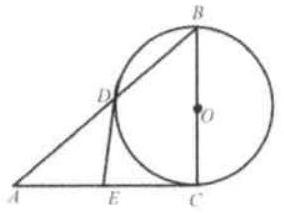
\includegraphics[width=\textwidth]{images/problem_image_1.jpg}
\end{center}

Connect \(C D\).\\
Since \(B C\) is the diameter, \(\angle B D C=\angle A D C=90^{\circ}\).


Let \(\angle B C D=\alpha, \angle C B D=\beta\).\\
So \(\angle A=\alpha, \angle E C D=\beta\).\\
Since both \(E D\) and \(E C\) are tangent to circle \(O, E D=E C\) and \(\angle E D C=\angle E C D=\beta\).\\
\centering
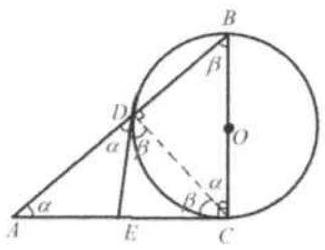
\includegraphics[width=\textwidth]{images/reasoning_image_1.jpg}

Thus \(\angle A D E=\alpha=\angle A\).\\
Triangle \(E A D\) is an isosceles triangle. So \(D E=A E\).\\

\end{document}
